\documentclass[a4paper,12pt]{article}
%\usepackage{fullpage}
%\usepackage{a4wide}
\usepackage[utf8]{inputenc}
\usepackage[danish, english]{babel}

% Nice looking font
%\usepackage{palatino}

% In order to highlight code
\usepackage[pdftex]{color}
\usepackage{listings}

% For graphics support
\usepackage{epsfig}
\usepackage{graphicx}
\usepackage{subfigure}

% Math support
\usepackage{amsmath}

% In order to include pdf
\usepackage{pdfpages}

% Graf support
%\usepackage{tkz-graph}

% Pdf section support
\usepackage{hyperref}
\hypersetup{
    bookmarks=true,         % show bookmarks bar?
    unicode=false,          % non-Latin characters in Acrobat's bookmarks
    pdftoolbar=false,       % show Acrobat's toolbar?
    pdfmenubar=false,       % show Acrobat's menu?
    pdffitwindow=true,      % page fit to window when opened
    pdftitle={OCamlCSP. A concurrency library for Ocaml}, % title
    pdfauthor={Joakim Ahnfelt-Rønne - 1986/03/14 - joakim.ahnfelt@gmail.com,
        Ramón Salvador Soto Mathiesen - 1979/05/15 - ramon@diku.dk and
        Advisor: Andrzej Filinski - andrzej@diku.dk}, % author
    pdfsubject={},   % subject of the document
    pdfnewwindow=true,      % links in new window
    pdfkeywords={keywords}, % list of keywords
    colorlinks=false,       % false: boxed links; true: colored links
    linkcolor=red,          % color of internal links
    citecolor=green,        % color of links to bibliography
    filecolor=magenta,      % color of file links
    urlcolor=cyan           % color of external links
}

% Macros
\newcommand{\missing}[1]{
\begin{tabular}{|p{11cm}|}
\hline
\emph{Missing:} {\scriptsize (things that need to be written or considered)} \\
\hline
#1
\hline
\end{tabular}
}

% ----------------------------------------------------------------------
% At skrive "%" betyder at man kommenterer ligesom som // i C, Java, osv
% ----------------------------------------------------------------------
% set up listing environment with C syntax hightlight
\definecolor{stringcolor}{rgb}{0.50,0.00,0.50}      %
\definecolor{commentcolor}{rgb}{0.00,0.50,0.00}     %
\definecolor{keywordcolor}{rgb}{0.00,0.00,1.00}     %
\definecolor{idcolor}{rgb}{0.00,0.00,0.00}          %
% with \lstset one can predefine parameters for listings
\lstset{language=ML,basicstyle=\ttfamily,keywordstyle=\color{keywordcolor},
        commentstyle={\color{commentcolor}\itshape},
        stringstyle={\color{stringcolor}},
        identifierstyle=\color{idcolor},numbers=left,
        xleftmargin=2em,% framerule=0.8pt,
        stepnumber=1,frame=tlrb,showstringspaces=false,
        firstnumber=1,numberstyle=\ttfamily, breaklines}
% ----------------------------------------------------------------------

% Opening
\title{OCamlCSP - a concurrency library for Ocaml}
\author{Joakim Ahnfelt-Rønne - 1986/03/14 - joakim.ahnfelt@gmail.com \and 
        Ramón Salvador Soto Mathiesen - 1979/05/15 - ramon@diku.dk \and
        \\ Advisor: Andrzej Filinski - andrzej@diku.dk}
\date{31$^{st}$ July 2009}

\begin{document}

\maketitle

\newpage

\selectlanguage{danish}
\begin{abstract}
% Grue: Højest 10 linjer: Hvad handler rapporten om? Hvilke resultater er
% opnået?
Her på dansk
\end{abstract}

\selectlanguage{english}
\begin{abstract}
Here in english
\end{abstract}

\newpage
\tableofcontents
\newpage

% Line breaks between paragraphs instead of indentation
\parindent=0pt
\parskip=8pt plus 2pt minus 4pt

\section{Introduction}
This project is a complete, designed and implemented, API for a CSP-based
concurrency library in a functional language, in this case Ocaml\cite{?}.

We have achieved our three primary goals we set at the beginning:
\begin{itemize}
 \item \textbf{Designing an API for a CSP-based concurrency library in a
     functional language}. Because our main focus was on the API design, most of
   the {\it Section} \ref{analysis} is related to this.
 \item \textbf{Implementing the concurrency API in a functional language.} A
   complete description on how we implemendted the API based on the limitations
   of the chosen language?, use of a global lock. For more information look in
   the {\it Section} \ref{implementation}.
 \item \textbf{Assessing the API and underlying implementation by comparing
     applications built on top of it with similar applications built on top of
     an existing CSP library}. We have made a simple CSP network, Fibonacci,
   and a more complex, Webproxy, in order to test the API. The application are
   similar to the applications we have made for one of the other CSP libraries.
   A full description on how these applications are build and how to compile-run
   can be seen in the {\it Section} \ref{test}.
\end{itemize}

The resulting API source code and documentation can be seen in the Appendix
\ref{appendixSrc} and \ref{appendixDoc}. A online version is also avaliable at:

\begin{center}
http://github.com/Ahnfelt/mlcsp/
\end{center}

About the possible extensions to this API, we got wise on that we cannot
implement true parallelism through system threads, see at {\it Section
\ref{analysis}} for more information, but how we ``maybe'' can implement
parallelism with distribution through sockets, see {\it Section 
\ref{conclusion}}.

\section{Analysis}
\label{analysis}
\missing{
- Are CSP channels any2any and bidirectional? \\
- Are CSP channels names or values? \\
- Why don't we provide CSP events? \\
- References to CSP and CSP libraries. \\
}

We would like our programs to resemble CSP in structure. In order to do that, we must
provide the synchronous bidirectional channels, alternation and processes.

For each construct, we are going to look at how it's done in CSP and CSP libraries,
how we would like to write it in OCaml, and what the semantics should be.

\subsection{Send \& receive}

Two of the basic constructs for CSP channels are send and receive:
\[c\,!\,e \to P\]
\[c\,?\,x \to Q(x)\]
Where $c$ is a channel, $e$ is an expression, $x$ is a name and $P$ and $Q$ are processes. 
The semantics of these are to synchronously send or receive a value respectively, and
then become another process. In the case of receive, the process may refer to the
received value $x$.

In PyCSP, these two constructs look like this:
\begin{verbatim}
c.write(e)
P
\end{verbatim}
\begin{verbatim}
x = c.read()
Q(x)
\end{verbatim}
It's using methods to realize the read/write, and sequence to realize \emph{becoming}
another process after the synchronization. Note that the channels are values, whereas
they are names in CSP. JCSP and C++CSP are similar.

The obvious way to look like CSP is to define operators ! and ? that works like the
CSP counterpart. However, it is not possible in OCaml to declare that the right hand 
side of the question mark introduces a binding. It is also not desireable to redefine
the special ! operator that is used for dereferencing mutable references in OCaml.

We therefore have to decide between methods and functions. The OCaml standard library
primarily uses functions to provide it's functionality, and few if any other ML 
variants share OCaml's object model. Since we don't anticipate any need for an
exstensible inheritance hierachy for channels, we choose functions for the task.
We use the \textbf{let in} construct to provide binding.

\begin{verbatim}
write c e; P
\end{verbatim}
\begin{verbatim}
let x = read c in Q(x)
\end{verbatim}

We are going to define the semantics of these in the next section.

\subsection{Alternation}
\missing{
- Wot? No chicken?\\
}

External choice in CSP looks like this:
\[(c_1\,?\,x \to P(x)\ |\ c_2\,?\,x \to Q(y)\ |\ c_3\,!\,e \to R)\]
Where there may be any number of processes separated by vertical bars.
The semantics is that the whole process becomes whichever of the listed processes 
that can take a step first. 

In PyCSP it looks like (where \texttt{in1 = c1.read}, \texttt{in2 = c2.read}, \texttt{out3 = c3.write}):
\begin{verbatim}
s = Alternative(in1, in2, out3).priSelect()
if s == in1:
    x = in1()
    P(x)
elif s == in2:
    y = in2()
    Q(y)
else:
    out3(e)
    R
\end{verbatim}

Note that the whole if-construct can be replaced by an application if all the guards have the same type 
and become the same process. The JCSP and C++CSP selects take in a list of guards and return the index
of the guard, which you can then switch on. In both cases, you have to \emph{promise} to read from the
chosen channel, or the behaviour will be undefined.

Starting from CSP's syntax, we might want to write something like \texttt{(A | B | C)}, where $A$, $B$
and $C$ are processes. If we consider processes functions of type $unit \to unit$ for this purpose, 
one might define an operator $|$ that takes two processes and returns the result of the one that is 
chosen. The problem with this is that it is very hard in plain OCaml to inspect functions at runtime to 
see which one of them can take a step.

Instead we make the first step inspectable by providing \emph{guards}, which is also the route taken by
the other libraries. However, we would like to avoid relying promises and idioms to obtain the 
intended behaviour. We therefore make the action an integral part of each guard. We use a list instead
of an operator in order to provide a more natural syntax for alternation with more than two choices.

\begin{verbatim}
select [
    read_guard c1 (fun x -> P(x));
    read_guard c2 (fun y -> Q(y));
    write_guard c3 e (fun _ -> R);
]
\end{verbatim}
Note that select also returns the result of the chosen action, which is particularily convenient if you
are reading and don't care which channel the value comes from.

In CSP, any process that can take a step may be chosen arbitrarily. However, if the same list of 
alternatives is used in a loop, this might lead to starvation. If one of the guards is always ready,
an arbitrary choice can be to chose this every time. This means that any other guards that are ready
will be skipped indefinatly, and thus be starved.

We solve this by prioritizing the guards in a random order each time select is called. That way the
chance that a ready guard is not taken approaches zero as the number calls to select grows. Note that
this is also a valid implementation of the arbitrary choice, which we don't provide separatly.

\subsection{Poison}
\missing{
What happens if some but not all alternatives in a select is poisoned? \\
}

\subsection{Omitted}
\missing{
- Internal choice, ``enabled'' array.\\
- Sequence.\\
- Polling. \\
- PriSelect.\\
- FairSelect from C++CSP? What is that. See C++csp/doc/guide2.html.1 \\
}

\subsection{Interface}

\subsubsection{Design}

\subsubsection{Comparison}

\begin{tabular}{l|l}
CSP & OCamlCSP \\
\hline
$c!e \to P$ & \texttt{write c e; P} \\
\hline
$c?x \to P(x)$ & \texttt{P (read c)} \\
\hline
$(a?x \to P(x)\ |\ b!e \to Q)$ 
&\verb|select [ read_guard a (fun x -> P(x)) ;| \\
&\verb|         write_guard b e (fun _ -> Q) ]|\\
\hline
$P \parallel Q$ 
&\verb|parallel [ (fun () -> P) ;| \\
&\verb|           (fun () -> Q) ]| \\
\end{tabular}

\missing{
- Occam \\
- PyCSP/JCSP/C++CSP \\
- Event \\
}


\section{Implementation}
\label{implementation}


\subsection{Channels}
A one to one channel is a channel that only allows one procees to read from it and one process 
to write to it. It may be implemented as a state machine as shown in figure \ref{channel-state}.
When the channel is in the NobodyWaiting state and a process tries to read from the channel,
it enters the ReaderWaiting state. When a writer comes along and tries to write to a channel
in this state, it returns to the NobodyWaiting state, transfers the message, and only then
allows the two processes to continue. The WriterWaiting state works in much the same way.

\begin{figure}[h]
\centering
\includegraphics[width=0.6\textwidth]{channel-state.png}
\caption{Simplified channel state (poison and multi-read/write not shown)}
\label{channel-state}
\end{figure}

From any state, the channel might be poisoned and enter the Poisoned state. If it was in the
ReaderWaiting or the WriterWaiting state, the waiting process will wake up and throw a special
exception. Any further attempts to read from or write to the channel will result in this 
exception being thrown again.

For any to any channels that places no restrictions on the number of processes that can read
from or write to it, we simply extend the above to keep a queue of readers (when in the 
ReaderWaiting state) or writers (when in the WriterWaiting state).

The choice of using a queue gives a stronger guarentee than CSP gives, namely that no processes
will be starved. By starvation we mean to say that a process waiting to read or write on the
channel can be blocked indefinately even though an infinite number of messages is transmitted
over the channel. This would happen with a stack if another process is always ready to read or 
write again before the channel was ready to accomodate the starving process. The starving process
would always be put behind the eager process with a stack, but with a queue, the starving process
will always advance in the queue every time a message is transmitted, guarenteeing that it will
eventually get it's turn.

In order to only wake up the waiting process, each process has it's own condition variable that
it waits on. Additionally, readers have a function that takes in a value and performs a side 
effect, while writers have a function that performs a side effect and produces a value. The side
effect for both is to set it's internal reference to the transmitted value (instead of None),
remove it from all the channels it's listening on and wake up the process.

We use a lock that is global to the library, in order to protect the channel and processes from
concurrent mutation. This lock is only ever taken when first trying to read from a channel, or
right after a process has been woken up. We claim that this won't lead to performance degradation,
since OCaml's threads only provides concurrency though time-sharing \cite{ocaml-threads}.

\missing{
- How do you get rid of this lock? (useful for porting). It is hard because you don't know which
channels you will touch before you have chosen a target process to transmit to/from. If you knew
that, you could simply take their locks in some well defined order (thus avoiding deadlock). \\
}

\begin{verbatim}
type 'a channel_state
    = NobodyWaiting 
    | ReaderWaiting of (Condition.t * ('a -> unit)) list
    | WriterWaiting of (Condition.t * (unit -> 'a)) list
    | Poisoned

type ('a, 'b) channel = ('a channel_state) ref
\end{verbatim}

The phantom type 'b is used for the channel permissions. This is enforced solely via the type
system, and is represented with a product of three booleans values: read * write * poison.
Reading, writing and poisoning are initially enabled for a channel, but handles with less 
permissions can be obtained through the functions shown in figure \ref{channel-permissions}. 
Permissions can only be taken away, not gained, which is evident from the types of the 
functions, for example: 

\begin{verbatim}
val read_poison_only : ('a, on * _ * on) channel -> 
                       ('a, on * off * on) channel
\end{verbatim}

Apart from the type, all of these functions are simply identity functions. We provide a
type alias \texttt{'a t = ('a, on * on * on) channel} for people who don't want to write the
longer (often optional) type annotations that the permission types incur.

\begin{figure}[h]
\centering
\begin{tabular}{c|c|c|l}
Read & Write & Poison & Function \\
\hline
0 & 0 & 0 & (useless) \\
0 & 0 & 1 & poison\_only \\
0 & 1 & 0 & write\_only \\
0 & 1 & 1 & write\_poison\_only \\
1 & 0 & 0 & read\_only \\
1 & 0 & 1 & read\_poison\_only \\
1 & 1 & 0 & read\_write\_only \\
1 & 1 & 1 & (default) \\
\end{tabular}
\caption{Channel permissions}
\label{channel-permissions}
\end{figure}

\subsection{Alternation}

\missing{
- Occam does not seem to sufficiently describe PRI ALT when two processes with inverse priorities
on the same two channels use it (in the manual). This is why we don't support it. \\
- Consider supporting something a bit like PRI ALT anyway since it's easier to build on top of
than the current randomized select. \\
}

\subsection{Processes}

\section{Test}

\label{test}
\begin{table}[ht]
\centering
\begin{tabular}{|c|c|c|c|}
    \hline
    	File name &
	Description &
	Expected Output &
	Run \\
    \hline
    	maxthreads.ml &
        &
        &
	OK \\
    \hline
    	nonblocking.ml &
        &
        &
	OK \\
    \hline
    	commstime.ml ??? &
        &
        &
	OK \\
    \hline
    	ssn.ml (numbers 0$\ldots$41) &
        &
        &
	OK \\
    \hline
    	ssn.ml (squares 0$\ldots$41) &
        &
        &
	OK \\
    \hline
\end{tabular} 
\caption{Test table ...}
\label{testtable}
\end{table}

\subsection{Fibonacci}


\subsection{Webproxy}


\section{Conclusion}
\label{conclusion}

If we compare how Brian Vinter teaches CSP\cite{vinter}:
\begin{center}
\begin{verbatim}
PairsInt (in, out) = Delta2Int (in, a, c) || 
                     TailInt (a, b) || 
                     PlusInt (b, c, out) 
\end{verbatim}
\end{center}

versus how we implement the simple network:

\begin{verbatim}
let pairsInt i o () =
  let a = Csp.channel () in
  let b = Csp.channel () in
  let c = Csp.channel () in
    Csp.parallel [
      delta2int i a c;
      tailint a b;
      plusint b c o;
    ]
\end{verbatim}

We can see that there is almost no difference beside the {\it parallel operator}
and definition of the channel variables.

% ----------------------------------------------------------------------
% Bibliography
% ----------------------------------------------------------------------
\begin{thebibliography}{99}

\bibitem[Hoare 04]{hoare}
:\\
Communicating Sequential Processes\\
C. A. R. Hoare\\
Prentice Hall International; (June 24, 2004)\\
ISBN-10: 0-13-153271-5\\
ISBN-13: 978-0-13-153271-7\\
http://www.usingcsp.com/cspbook.pdf

\bibitem[Vinter, CSP]{vinter}
:\\
Threading\\
Brian Vinter\\
Department of Computer Science. University of Copenhagen\\
http://isis.ku.dk/kurser/blob.aspx?feltid=224185\\
Last visited: $20^{th}$ july 2009



\end{thebibliography}
% ----------------------------------------------------------------------


\appendix
\newpage
\section{Appendix: Source code}
\label{appendixSrc}

\scriptsize
\subsection{API}
\label{appendixAPI}
\subsubsection{Interface (.mli)}
\lstinputlisting{../source/csp.mli}
\subsubsection{Source (.ml)}
\lstinputlisting{../source/csp.ml}
\subsection{CSP Library (Legoland)}
\lstinputlisting{../source/legoland.ml}
\normalsize

\section{Appendix: Documentation}
\label{appendixDoc}
\begin{center}
  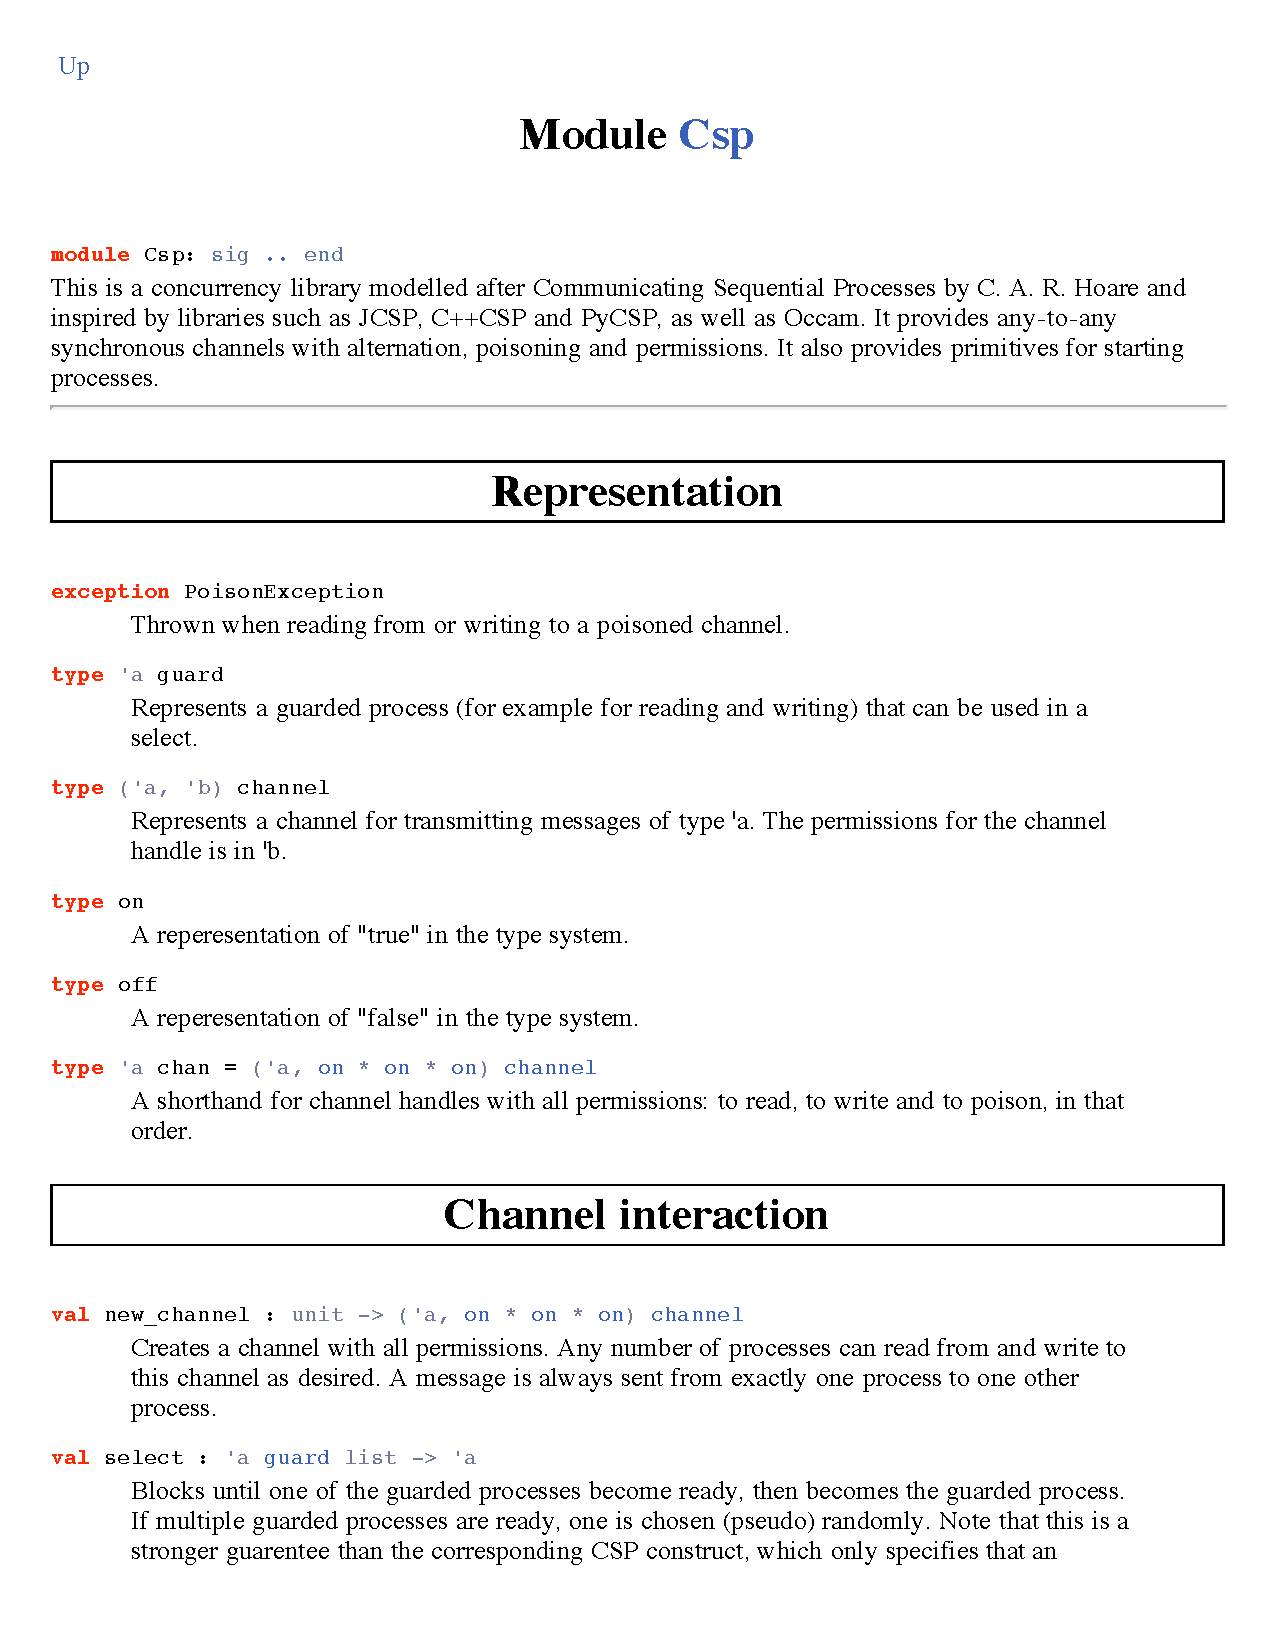
\includepdf[pages=-]{../docs/csp.pdf}
\end{center}


\newpage
\section{Appendix: Test}
\label{appendixTest}
\scriptsize
\subsection{Fibonacci}
\lstinputlisting{../test/fibCSP.ml}

\subsection{Webproxy}
\lstinputlisting{../test/proxyCSP.ml}
\normalsize

\end{document}
